\documentclass[12pt,a4paper]{article}

\usepackage{fontawesome5}
\providecommand{\faPencilAlt}{\faIcon{pencil-alt}}

\usepackage{styles/couleurs}
\usepackage{styles/mise_en_page}
\usepackage{styles/boites}
\usepackage{styles/maths}
\usepackage{styles/figures}

\usepackage{enumitem}
\usepackage{array}
\usepackage{tabularx}
\usepackage{amsmath}
\usepackage{amssymb}
\usepackage{tikz}
\usepackage{xparse}

\usetikzlibrary{calc,angles,quotes,arrows.meta}

\setlist[itemize]{leftmargin=1.4em,itemsep=0.15em,topsep=0.2em}
\setlist[enumerate]{leftmargin=*,itemsep=0.22em,topsep=0.25em}

\newcommand{\lignepointillee}{\noindent\dotfill\par\vspace{0.45em}}

\newcommand{\lignesreponse}[1]{%
\begin{tcolorbox}[
enhanced,colback=white,colframe=NeutreC!40,boxrule=0.5pt,arc=1.5mm,
left=3mm,right=3mm,top=2mm,bottom=1mm,before skip=2pt,after skip=2pt]
\foreach \i in {1,...,#1}{\lignepointillee}
\end{tcolorbox}}

\newcommand{\titreseq}[1]{%
\begin{center}
{\sffamily\LARGE\bfseries\color{TitreC}Séquence 6 -- Cosinus d'un angle aigu}\\[0.2em]
{\sffamily\large\bfseries\color{SavoirC}#1}
\end{center}}

\begin{document}

\titreseq{Activité 1 -- Quel outil pour calculer une longueur ?}

\remarque{Cette activité sert de diagnostic. Le but n'est pas encore d'utiliser le cosinus,
mais de distinguer ce que l'on sait déjà faire de ce qui nécessite un nouvel outil.}

\section*{Partie A -- Rappels sur le triangle rectangle}

\begin{center}
\begin{tikzpicture}[scale=0.95]
  \coordinate (A) at (0,0);
  \coordinate (B) at (4.2,0);
  \coordinate (C) at (4.2,2.8);

  \draw[line width=0.9pt] (A)--(B)--(C)--cycle;
  \draw (3.85,0)--(3.85,0.35)--(4.2,0.35);

  \node[left] at (A) {$A$};
  \node[below] at (B) {$B$};
  \node[above] at (C) {$C$};

  \draw[ActionC,line width=1pt] (0.7,0) arc[start angle=0,end angle=34,radius=0.7];
  \node[ActionC] at (1.05,0.35) {$\widehat{A}$};
\end{tikzpicture}
\end{center}

\begin{enumerate}
  \item En quel point le triangle est-il rectangle ?
  \item Quel côté est l'hypoténuse ?
  \item Parmi les deux côtés de l'angle \(\widehat A\), lequel n'est pas l'hypoténuse ?
  \item Si l'on étudiait l'angle \(\widehat C\), le même côté serait-il choisi ?
\end{enumerate}

\lignesreponse{5}

\section*{Partie B -- Deux longueurs à calculer}

\begin{minipage}[t]{0.48\textwidth}
\vspace{0pt}
\textbf{Situation 1}

\begin{center}
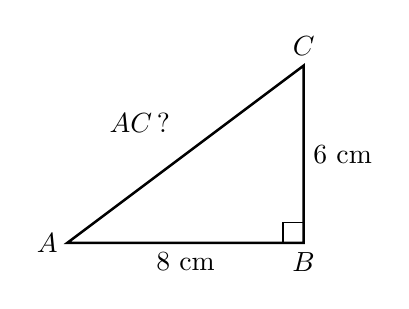
\begin{tikzpicture}[scale=0.75]
  \coordinate (A) at (0,0);
  \coordinate (B) at (4,0);
  \coordinate (C) at (4,3);

  \draw[line width=0.9pt] (A)--(B)--(C)--cycle;
  \draw (3.65,0)--(3.65,0.35)--(4,0.35);

  \node[left] at (A) {$A$};
  \node[below] at (B) {$B$};
  \node[above] at (C) {$C$};

  \node[below] at (2,0) {$8$ cm};
  \node[right] at (4,1.5) {$6$ cm};
  \node[above left] at (1.9,1.7) {$AC\,?$};
\end{tikzpicture}
\end{center}

Peut-on calculer \(AC\) avec un outil déjà connu ?
Nomme cet outil et effectue le calcul.
\end{minipage}
\hfill
\begin{minipage}[t]{0.48\textwidth}
\vspace{0pt}
\textbf{Situation 2}

\begin{center}
\begin{tikzpicture}[scale=0.75]
  \coordinate (D) at (0,0);
  \coordinate (E) at (4.2,0);
  \coordinate (F) at (4.2,2.8);

  \draw[line width=0.9pt] (D)--(E)--(F)--cycle;
  \draw (3.85,0)--(3.85,0.35)--(4.2,0.35);

  \node[left] at (D) {$D$};
  \node[below] at (E) {$E$};
  \node[above] at (F) {$F$};

  \node[above left] at (2.15,1.55) {$10$ cm};
  \node[below] at (2.2,0) {$DE\,?$};

  \draw[ActionC,line width=1pt] (0.75,0) arc[start angle=0,end angle=34,radius=0.75];
  \node[ActionC] at (1.1,0.38) {$35^\circ$};
\end{tikzpicture}
\end{center}

Peut-on appliquer directement le théorème de Pythagore ?
Explique ce qui manque.
\end{minipage}

\lignesreponse{7}

\section*{Partie C -- Estimer avant de calculer}

Sans connaître encore la méthode exacte, encadre la longueur \(DE\).

\[
0<DE<\ldots
\]

Parmi \(2\) cm, \(8\) cm, \(12\) cm et \(20\) cm,
quelles valeurs sont impossibles ? Justifie.

\lignesreponse{4}

\section*{Partie D -- La nouvelle question}

Complète la phrase qui guidera la suite de la séquence.

\begin{tcolorbox}[colback=SavoirC!5,colframe=SavoirC!60,boxrule=0.7pt,arc=2mm]
Dans un triangle rectangle, comment calculer un côté de l'angle droit
lorsque l'on connaît l'\dotfill{} et un \dotfill{} aigu ?
\end{tcolorbox}

\end{document}
